% Figure: roadmap timeline (part 11).
% Build: pdflatex roadmap_timeline.tex  (run inside figures/)
\documentclass[tikz,border=6pt]{standalone}
\usetikzlibrary{positioning,arrows.meta}
\begin{document}
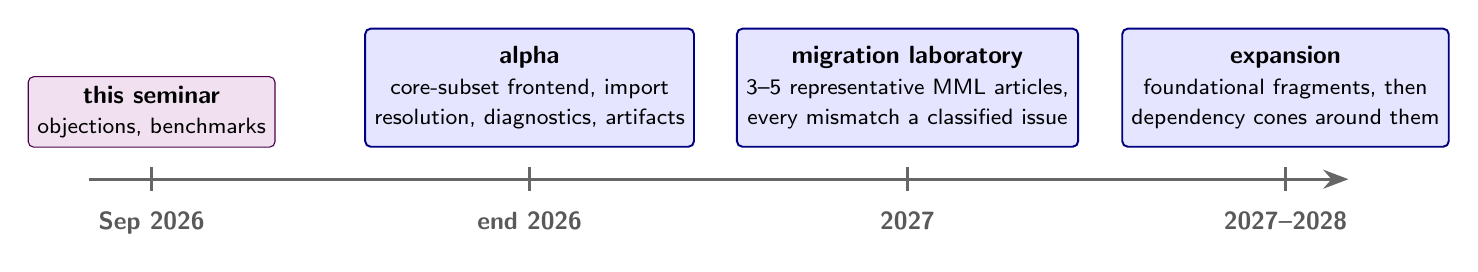
\begin{tikzpicture}[
  font=\sffamily,
  phase/.style={draw, rounded corners=2pt, align=center, minimum width=40mm,
                minimum height=15mm, line width=0.7pt, fill=blue!10,
                draw=blue!50!black, font=\sffamily\small},
  when/.style={font=\sffamily\small\bfseries, text=black!65},
  axis/.style={-{Stealth[length=3.2mm]}, line width=1.2pt, black!60},
  tick/.style={line width=1pt, black!60},
]
  \draw[axis] (-8mm,0) -- (152mm,0);

  % Seminar marker
  \draw[tick] (0mm,-1.5mm) -- (0mm,1.5mm);
  \node[when, below=3mm of {(0mm,0)}] {Sep 2026};
  \node[draw, rounded corners=2pt, fill=violet!12, draw=violet!60!black,
        align=center, font=\sffamily\small, above=4mm of {(0mm,0)}]
    {\textbf{this seminar}\\ \footnotesize objections, benchmarks};

  % Alpha
  \draw[tick] (48mm,-1.5mm) -- (48mm,1.5mm);
  \node[when, below=3mm of {(48mm,0)}] {end 2026};
  \node[phase, above=4mm of {(48mm,0)}]
    {\textbf{alpha}\\ \footnotesize core-subset frontend, import\\
     \footnotesize resolution, diagnostics, artifacts};

  % Migration lab
  \draw[tick] (96mm,-1.5mm) -- (96mm,1.5mm);
  \node[when, below=3mm of {(96mm,0)}] {2027};
  \node[phase, above=4mm of {(96mm,0)}]
    {\textbf{migration laboratory}\\ \footnotesize 3--5 representative MML
     articles,\\ \footnotesize every mismatch a classified issue};

  % Expansion
  \draw[tick] (144mm,-1.5mm) -- (144mm,1.5mm);
  \node[when, below=3mm of {(144mm,0)}] {2027--2028};
  \node[phase, above=4mm of {(144mm,0)}]
    {\textbf{expansion}\\ \footnotesize foundational fragments, then\\
     \footnotesize dependency cones around them};
\end{tikzpicture}
\end{document}
